\chapter{Results}

\epigraph{\centering ``It is really rather strange that human beings are normally deaf to the strongest arguments
while they are always inclined to overestimate measuring accuracies.''}{--- Albert Einstein}

OXYGEN CONSUMPTION: The uteri of forty-six animals, twenty-three young and twenty-three senescent, were studied by the Gilson
manometric technique, and six (three young, three old) by the Beckman oxygen electrode method. The mean QO$_{2}$ (in $\mu$g O$_{2}$/mg. wet
weight/hour) were:

\begin{center}
  \begin{tabular*}{0.8\linewidth}{@{\extracolsep{\fill}} c  c  c}
    Senescent &  Young & P \\
    3.7 & 2.5 & <0.05 \\
  \end{tabular*}
\end{center}

This is not a high level of significance, but the limitation is probably inherent in the method (Jusiak, 1970). Finer discrimination can be
achieved by using an indirect method such as TTC reduction, assuming that these two events closely correspond to each other, as indicated
by Cascarano and Zweifach (1955). The problem of ammonia production will be discussed below (under Oxygen Consumption, in Discussion).

LUMINAL OXYGEN TENSION: Cycling animals:

\begin{center}
  \begin{tabular*}{0.8\linewidth}{@{\extracolsep{\fill}} c c  c  c}
    ~ & Senescent (5) & Young (5) & Vitamin E treated (3) \\
    Range, & 0-2 & 4-8 & 6-12 \\
    mm Hg & ~ & ~ & ~ \\
  \end{tabular*}
\end{center}

The oxygen tensions measured in the senescent uteri are in the range known to limit \textit{in vitro} respiration, and also to limit development
of cultured embryos (Needham, 1931), but the exact oxygen requirements of embryos are not accurately known, since oxygen tension is normally
measured only in the gas phase. The effective Km for oxygen increases with increased cell diameter (Longmuir, 1957), and the viscosity of the
surrounding medium must also have an effect. The early period following ovulation is likely to be similar in both the regular cycle and following
mating. This difference in pO$_{2}$ could easily account for the early retardation observed in senescent hamsters' embryos, such as lagging cleavage and delay
in loss of the zona pellucida. The established lag in uterine changes (Connors, 1969; Stockton, 1972) suggests that this difference in pO$_{2}$ may become
even more distinct around the time of implantation, when respiration is even higher, and the likelihood of damage even greater, but the fact that the
lumen no longer exists at this time makes it necessary to depend on indirect evidence. If it can be generally accepted that TTC reduction does accurately
reflect the QO$_{2}$ of a tissue, then a complete study of the differences in uterine reductive capacity between old and young animals should be done on
each day of pregnancy, to build on the very suggestive work that has been done on rats of different ages by Schultze (1967).

One young and one senescent hamster on day 4$\frac{1}{2}$ of pregnancy were used in an attempt to study the luminal oxygen tension directly, and the
pO$_{2}$s measured were 4 mm Hg in the senescent, and 15-40 mm Hg in the young. However, the procedure caused tremendous disruption of the tissues. Since
the closure of the young lumen is believed to be firmer than that of the old animal, this very large difference could probably be at least partly attributed
to greater bleeding in the young. Nevertheless, differences such as these would be expected on the basis of decreased oxygen consumption of implantation
sites, and the senescent lag in factors related to implantation.

TTC REDUCTION:

\begin{center}
  \begin{tabular*}{0.8\linewidth}{@{\extracolsep{\fill}} c c  c  c}
    ~ & Senescent & Young & P \\
    \% Transmittance & 33 & 48 & <0.01 \\
    at 475 nm. & ~ & ~ & ~ \\
  \end{tabular*}
\end{center}

These values are equivalent to approximately 0.05 and 0.03 mg. formazan per sample, respectively (22 animals). In a group of three yound litter mates
and three old litter mates, the variability was much less (P <0.001).

$\beta$-GLUCURONIDASE: Mean \% transmittance at 540 nm. after one hour incubation:

\begin{center}
  \begin{tabular*}{0.8\linewidth}{@{\extracolsep{\fill}} c c  c}
    Senescent (3) & Young (3) & P\\
    34 & 20 & <0.01
  \end{tabular*}
\end{center}

Sections showed a generalized pale stain, except around blood vessels, where it was very intense.

PEROXIDASE: Mean \% transmittance at 540 nm. and at 90 seconds:

\begin{center}
  \begin{tabular*}{0.8\linewidth}{@{\extracolsep{\fill}} c c c}
    Senescent (4) & Young (4) & P\\
    59 & 66 & <0.05
  \end{tabular*}
\end{center}

Sections showed intensely stained granules about 5 $\mu$ in diameter distributed throughout, but especially in the endometrium, and a
very intensely stained endometrial epithelium; a few larger areas, about 20 by 80 microns, were more lightly stained; these may have been blood vessels.

CATALASE: Mean $\mu$l O$_{2}$ at 5 minutes:

\begin{center}
  \begin{tabular*}{0.8\linewidth}{@{\extracolsep{\fill}} c c c}
    Senescent (4) & Young (4) & P\\
    78 & 105 & <0.05
  \end{tabular*}
\end{center}

UTERINE WEIGHT:

\begin{center}
  \begin{tabular*}{0.8\linewidth}{@{\extracolsep{\fill}} c c c c}
    ~ & 3-6 Months & 14 Months & P\\
    Mean & 385 mg. & 592 mg. & <0.001
  \end{tabular*}
\end{center}

Mean ratio dry weight/wet weight:

\begin{center}
  \begin{tabular*}{0.8\linewidth}{@{\extracolsep{\fill}} c c c c}
    ~ & ~ & Senescent & Young\\
    25 Animals & Myometrium & 1:4 & 1:6\\
    12 Animals & Endometrium & 1:6.5 & 1:6.6
  \end{tabular*}
\end{center}

The greatest increase of thickness was in the myometrium, but the endometrium also appeared to become thicker with age.

\section{Estrogen Assays}

BROWN-ITTRICH FLUORESCENSE METHOD: Five old and three young uteri showed a significant difference in fluorescence at the frequencies
used for the oxidation product (or products) of estrogen. The shape of the spectrum was similar to that of estrogen products, and to
that of the standard solutions used, within the resolution, which was very poor under these conditions of sensitivity and frequency.

Mean intensity of fluorescence (in arbitrary units):

\begin{center}
  \begin{tabular*}{0.8\linewidth}{@{\extracolsep{\fill}} c c c}
    Mean S (5) & Mean Y (3) & P\\
    52 & 14 & <0.01
  \end{tabular*}
\end{center}

\begin{center}
Estradiol Standard
\end{center}

\begin{center}
  \begin{tabular*}{0.8\linewidth}{@{\extracolsep{\fill}} c c}
    1 $\mu$g & 10 $\mu$g\\
    19 & 27
  \end{tabular*}
\end{center}

DYE COUPLING METHOD (4-amino-6-chloro-m-benzenedisulfonamide): Rather than the red product resulting from condensation of estrogen
with the dye, both young and old gave a yellow product; the old gave a more intense yellow color. This would suggest either that there
was no estrogen in the extract, or that there were other materials that condensed with the dye more easily. The technique was discarded
as an estrogen assay, but the fact that there was an age-dependent difference, and that bile pigments similarly condense to form diazo
products, suggest that the product's spectrum should be compared with known bile pigments similarly condensed.

BIOASSAY: Since this method was intended to assay for ``estrogenicity'' bound in the uterus, extraction was made in acetone, in which estrogen
is highly soluble. An effect on the uterine weight was the intended object of investigation. However, it was noticed that after two injections
(containing the extract of $\frac{1}{2}$ an old uterus) the ovariectomized recipient had red fluorescence around one eye. This typical Harderian
fluorescence has been reported not to occur in ovariectomized animals unless estrogen has been administered, althrough injection of porphyrins into
intact rodents can cause increased secretion, which has led to the concept that the gland may concentrate and secrete porphyrins produced elsewhere, rather
than synthesizing them (Figge, 1947). No difference in uterine weight was observed.

AGE PIGMENT: The age pigment spectrum of certain tissues has been studied by Strehler (1976) and Karnaukhov (1971). Strehler reported increasing
but homogenous absorbtion at higher frequency ultraviolet, but Karnaukhov found several peaks of absorbtion around 260-280 nm. (an acetone extract
in petroleum ether) in nerve and salivary gland extracts. The uterine pigment, extracted in ether, shows increasing absorbtion at shorter wavelength
(especially below 250 nm.), except for a peak at 280 nm., similar to one observed in a blood extract and to one peak in Karnaukhov's extract. This is
consistent with the suggestion of Orsini and Meyer (1962) and Deno (1937) that the pigment is related to blood or hemosiderin, but the nearly smooth
absorbtion curve could represent a complex mixture. The peak at 280 nm. is lost in a methanol extract.

\noindent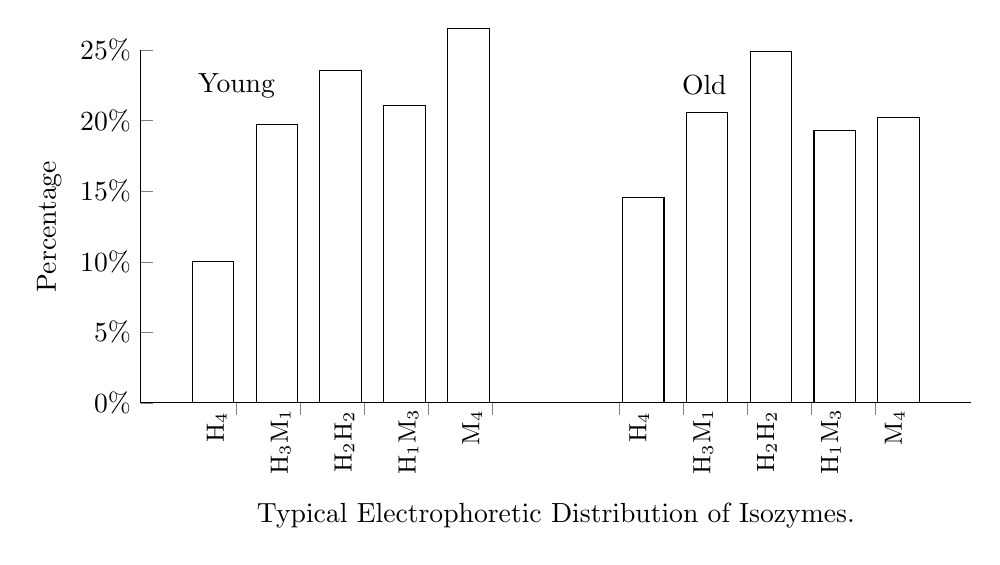
\begin{tikzpicture}
\begin{axis}[
    ybar,
    bar width=15pt,
    enlarge x limits=0.15,
    ylabel={Percentage},
    xlabel={Typical Electrophoretic Distribution of Isozymes.},
    ytick={0,5,10,15,20,25},
    yticklabels={0\%,5\%,10\%,15\%,20\%,25\%},
    ymin=0,
    ymax=25,
    axis lines*=left,
    xtick={1,2,3,4,5,7,8,9,10,11},
    xticklabels={,,,,,,,,,,}, 
    x tick label style={font=\small},
    width=\linewidth,
    height=0.5\linewidth,
    legend style={draw=none},
    clip=false,
    xlabel style={yshift=-5ex}
]

\addplot[fill=white, draw=black] coordinates {
    (1,10.042735042735043)  
    (2,19.71153846153846)  
    (3,23.55769230769231)   
    (4,21.04700854700855)  
    (5,26.549145299145305)   
};

\addplot[fill=white, draw=black] coordinates {
    (7,14.529914529914532)  
    (8,20.566239316239322)  
    (9,24.893162393162395)  
    (10,19.284188034188038) 
    (11,20.219017094017094)  
};

\node[rotate=90, anchor=south] at (axis cs:1,-1.75) {\small $\mathrm{H}_4$};
\node[rotate=90, anchor=south] at (axis cs:2,-2.75) {\small $\mathrm{H}_3\mathrm{M}_1$};
\node[rotate=90, anchor=south] at (axis cs:3,-2.75) {\small $\mathrm{H}_2\mathrm{H}_2$};
\node[rotate=90, anchor=south] at (axis cs:4,-2.75) {\small $\mathrm{H}_1\mathrm{M}_3$};
\node[rotate=90, anchor=south] at (axis cs:5,-1.75) {\small $\mathrm{M}_4$};

\node[rotate=90, anchor=north] at (axis cs:7,-1.75) {\small $\mathrm{H}_4$};
\node[rotate=90, anchor=north] at (axis cs:8,-2.75) {\small $\mathrm{H}_3\mathrm{M}_1$};
\node[rotate=90, anchor=north] at (axis cs:9,-2.75) {\small $\mathrm{H}_2\mathrm{H}_2$};
\node[rotate=90, anchor=north] at (axis cs:10,-2.75) {\small $\mathrm{H}_1\mathrm{M}_3$};
\node[rotate=90, anchor=north] at (axis cs:11,-1.75) {\small $\mathrm{M}_4$};

\node at (axis cs:1,22.5) {Young};
\node at (axis cs:8.325,22.5) {Old};

\end{axis}
\end{tikzpicture}

\begin{center}
  Mean \% of H$_{4}$:
\end{center}

\begin{center}
  \begin{tabular*}{0.8\linewidth}{@{\extracolsep{\fill}} c c c c}
    ~ & S & Y & P\\
    12 Animals & 14.3 & 10.7 & 0.05\\
    (6 old, 6 & ~ & ~ & ~\\
    young) & ~ & ~ & ~
  \end{tabular*}
\end{center}

\begin{center}
  Total LDH Activity in B-B Units per ml.:
\end{center}

\begin{center}
  \begin{tabular*}{0.8\linewidth}{@{\extracolsep{\fill}} c c c}
    S & Y & P\\
    1700 & 1950 & 0.05
  \end{tabular*}
\end{center}

\noindent\begin{tikzpicture}
\begin{axis}[
    height=1.5\textwidth,
    width=\textwidth,
    axis x line=bottom,
    axis y line=left,
    axis line style={-},
    enlarge x limits=0.05,
    xmode=log,
    ymode=log,
    xmin=512,
    xmax=16384,
    ymin=1,
    ymax=7,
    ytick={1,2,3,4,5,6,7},
    yticklabels={1,2,3,4,5,6,7},
    xtick={512,1024,2048,4096,8192},
    xticklabels={2$^{9}$,2$^{10}$,2$^{11}$,2$^{12}$,2$^{13}$},
    minor tick num=0,
    xlabel={Time},
    ylabel={Amplitude}
]

\addplot[only marks, mark=*, mark size=1pt, color=black] coordinates {
(484.473392796994, 5.154371404524182)
(583.7664022298974, 4.631726306379266)
(692.7033586920346, 4.124722936292416)
(989.5959201130876, 3.56152022889325)
(1858.9321760543821, 2.553555376667845)
(2065.2799963287357, 2.4881773489912424)
(8732.88089123549, 1.0845901137960103)
};

\addplot[no markers, black, thick] table [
            y={create col/linear regression={y=Y}},
        ] {
            X Y
484.473392796994 5.154371404524182
583.7664022298974 4.631726306379266
692.7033586920346 4.124722936292416
989.5959201130876 3.56152022889325
1858.9321760543821 2.553555376667845
2065.2799963287357 2.4881773489912424
8732.88089123549 1.0845901137960103
        }; 

\addplot[only marks, mark=*, mark size=1pt, color=black] coordinates {
(476.6543885636081, 5.555944992854687)
(581.3915572955749, 5.063046392407869)
(704.8402424186651, 4.577074560598036)
(994.4981823178825, 3.9798454712667004)
(2030.4584265600981, 2.865102603754915)
(2201.54328499399, 2.709153812211149)
(8766.200585647728, 1.342192620230919)
};

\addplot[no markers, black, thick] table [
            y={create col/linear regression={y=Y}},
        ] {
            X Y
476.6543885636081 5.555944992854687
581.3915572955749 5.063046392407869
704.8402424186651 4.577074560598036
994.4981823178825 3.9798454712667004
2030.4584265600981 2.865102603754915
2201.54328499399 2.709153812211149
8766.200585647728 1.342192620230919
        }; 


\addplot[only marks, mark=*, mark size=1pt, color=black] coordinates {
(484.5533808541257, 6.705770062873648)
(562.3578003154925, 6.290533457111426)
(698.7598691365937, 5.726809780461477)
(1020.1143273528011, 4.920255941710608)
(2477.908979070812, 3.2897529295615016)
(8624.803425059117, 1.9087671087524056)
};

\addplot[no markers, black, thick] table [
            y={create col/linear regression={y=Y}},
        ] {
            X Y
484.5533808541257 6.705770062873648
562.3578003154925 6.290533457111426
698.7598691365937 5.726809780461477
1020.1143273528011 4.920255941710608
2477.908979070812 3.2897529295615016
8624.803425059117 1.9087671087524056
        }; 




    \draw [shorten >=2.5pt, shorten <=5pt] (7155.206427666167, 1.2587612021305639) -- ++(0:1cm) 
    node[
      anchor=west,
      align=left,
      text depth=0ex,
      inner sep=0pt,
      line width=1pt
    ] {Young};

        \draw [shorten >=2.5pt, shorten <=5pt] (5332.0033277324565, 1.7861805824247037) -- ++(0:1cm) 
    node[
      anchor=west,
      align=left,
      text depth=0ex,
      inner sep=0pt,
      line width=1pt
    ] {Estrogen};

        \draw [shorten >=2.5pt, shorten <=5pt] (8281.06371761685, 2.002608639918147) -- ++(0:1cm) 
    node[
      anchor=west,
      align=left,
      text depth=0ex,
      inner sep=0pt,
      line width=1pt
    ] {Old};

            \draw [shorten >=2.5pt, shorten <=5pt] (2477.908979070812, 3.2897529295615016) -- ++(20:1cm) 
    node[
      anchor=west,
      align=left,
      text depth=0ex,
      inner sep=0pt,
      line width=1pt
    ] {Half Time};

   \node at (rel axis cs:0.5,0.95) {NMR Spin Echo of Whole Uteri};

   \node at (rel axis cs:0.5,0.925) {(Absolute amplitude is only an effect of sample size.)};

\end{axis}
\end{tikzpicture}

\begin{center}
  Harderian fluorescence:
\end{center}

\begin{center}
\noindent\hspace*{-0.175\linewidth}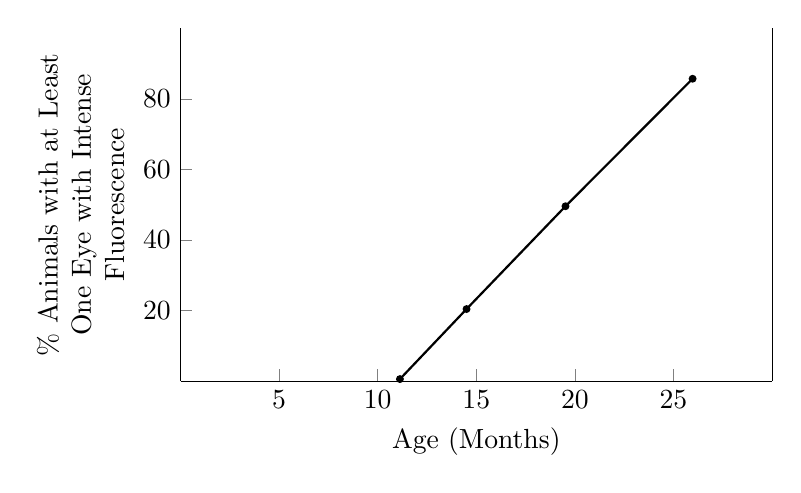
\begin{tikzpicture}
\begin{axis}[
    width=0.75\linewidth,
    height=0.5\linewidth,
    axis lines*=box,
    axis x line*=bottom,
    axis line style={-},
    xtick={5,10,15,20,25},
    ytick={20,40,60,80},
    ytick pos=left,
    xmin=0, xmax=30,
    ymin=0, ymax=100,
    ylabel={\% Animals with at Least\\One Eye with Intense\\Fluorescence},
    xlabel={Age (Months)},
    ylabel style={align=center},
    clip=false
]

\addplot[mark=*, mark size=1pt, thick] coordinates {
    (11.127879886098887, 0.5627750453016063)
    (14.505565622573128, 20.409008542583493)
    (19.524203986538957, 49.546725342997675)
    (25.970748123220297, 85.67952368625423)
};

\end{axis}
\end{tikzpicture}

\end{center}

Approximate incidence of red eye fluorescence with age in months. 25 animals.

\begin{center}
NMR Spin Echo:
\end{center}

The NMR spin echo results are similar to those of Damadian
(1971) comparing tumor with normal tissue, and of Hazelwood (1971),
comparing fetal with mature tissue. The results suggest that
senescent uterine water is more bulk-like than that of young uterus,
as tumor and fetal tissue water is more bulk-like than that of normal
and mature tissues.